\input{../.preambles/03-questions}
\input{../.preambles/10-russian}
\input{../.preambles/20-math}

\newcommand{\up}{\uparrow}
\newcommand{\down}{\downarrow}
\newcommand{\updown}{\up\down}
\newcommand{\ds}{\displaystyle}

\begin{document}
\def\contentsname{Список вопросов}
\tableofcontents
\newpage
\emph{1. Способы задания движения материальной точки. Векторный и координатный
способы задания движения. Определение траектории движения, скорости, ускорения.}

\vspace*{1em}
Существует три способа задания движения точки: естественный, векторный и
координатный. Остановимся на двух последних.

\header{Векторный способ задания движения}
\begin{table}[h!]
    \begin{tabular}{C{.4}m{.55\textwidth}}
        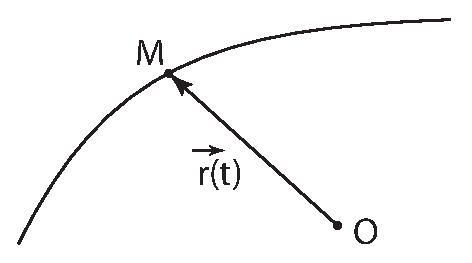
\includegraphics[width=.4\textwidth]{1_vect} &
        Положение точки в пространстве однозначно определяется заданием
        радиус-вектора \( \vec{r} \), проведенного из некоторого неподвижного
        центра \( O \) в данную точку \( M \).
        
        Для определения движения точки нужно знать как меняется с течением
        времени радиус-вектор \( \vec{r} \), то есть должна быть задана
        вектор-функция
    \end{tabular}
\end{table}

аргумента \( t \):
\[
    \vec{r} = \vec{r}(t).
\]

Траектория движения представляет собой геометрическое место концов
радиус-вектора \( \vec{r} \) движущейся точки.

\header{Координатный способ задания движения}

Рассмотрим движение точки \( M \) в трехмерном пространстве. Введем
прямоугольные декартовы координаты \( Oxyz \). Тогда в системе отсчета
\( Oxyz \) положение точки \( M \) определяется тремя координатами
\( (x, y, z) \). При движении точки \( M \) ее координаты изменяются с течением
времени. Следовательно:
\[ \left\{ \begin{array}{l}
    x = f_1(t); \\
    y = f_2(t); \\
    z = f_3(t).
\end{array} \right. \]

Эти уравнения называются уравнениями движения точки в декартовых координатах. Их
можно рассматривать как параметрические уравнения траектории точки. При
исключении параметра \( t \) из уравнений движения получаются уравнения
траектории в координатной форме.

Так, решив первое уравнение относительно \( t \), получим \( t = \phi(x) \).
Подставив полученное выражение для \( t \) в два других уравнения, получаем
уравнения траектории точки в координатной форме:
\[ \left\{ \begin{array}{l}
    x = f_1[\phi(x)]; \\
    y = f_2[\phi(x)].
\end{array} \right. \]
Координатный способ может быть получен из векторного проецированием на орты, так
как имеет место представление радиус-вектора:
\[
    \vec{r}(t) = x(t)\cdot\vec{e}_x + y(t)\cdot\vec{e}_y + z(t)\cdot\vec{e}_z.
\]

\header{Скорость}

Скорость -- это векторная величина, характеризующая быстроту и направление
движения точки в данной системе отсчета. При векторном способе задания движения
скорость:
\[
    \vec{v} \defeq \lim_{\D t \to 0} \Der{\vec{r}}{t} = \der{\vec{r}}{t}.
\]

Из определения следует, что скорость является производной по времени от радиус
вектора и направлена по касательной к траектории в сторону движения точки.

Для координатного способа получим (в декартовых координатах):
\[
    \vec{v} = \der{\vec{r}}{t} = \der{}{t}\Big(x(t)\cdot\vec{e}_x +
    y(t)\cdot\vec{e}_y + z(t)\cdot\vec{e}_z\Big) = \der{x}{t}\cdot\vec{e}_x +
    \der{y}{t}\cdot\vec{e}_y + \der{z}{t}\cdot\vec{e}_z = v_x\cdot\vec{e}_x +
    v_y\cdot\vec{e}_y + v_z\cdot\vec{e}_z.
\]

Следовательно, проекции скорости точки на неподвижные оси декартовых координат
равны первым производным от соответствующих координат точки по времени.

Модуль скорости и её направление можно определить, зная проекции:
\[
    v = \sqrt{v_x^2 + v_y^2 + v_z^2}, \quad
    \cos\left(\vec{v}, \vec{e}_x\right) = \frac{v_x}{v},\ \ 
    \cos\left(\vec{v}, \vec{e}_y\right) = \frac{v_y}{v},\ \ 
    \cos\left(\vec{v}, \vec{e}_z\right) = \frac{v_z}{v}.
\]

\header{Ускорение}

При неравномерном криволинейном движении точки изменяются модуль и направление
её скорости. Ускорение точки характеризует быстроту изменения модуля и
направления скорости точки.
\[
    \vec{a} \defeq \lim_{\D t \to 0} \Der{\vec{v}}{t} = \der{\vec{v}}{t} =
    \dder{\vec{r}}{t}.
\]

Вектор ускорения направлен по касательной к годографу скорости, расположен в
соприкасающейся плоскости и направле в сторону вогнутости кривой.

Как и в случае со скоростью, можно перейти к координатам. Получим:
\begin{align*}
    a_x = \dder{x}{t},\ \ a_y & = \dder{y}{t},\ \ a_z = \dder{z}{t}; \\
    a = \sqrt{a_x^2 + a_y^2 + a_z^2}, \quad
    \cos\left(\vec{a}, \vec{e}_x\right) = \frac{a_x}{a}, & \ \ 
    \cos\left(\vec{a}, \vec{e}_y\right) = \frac{a_y}{a},\ \ 
    \cos\left(\vec{a}, \vec{e}_z\right) = \frac{a_z}{a}.
\end{align*}

\newpage % ---------------------------------------------------------------------

\question{Эффект Шоттки. Его влияние на эмиссию электронов}
Эффект Шоттки состоит в возрастании тока в диоде при увеличении напряжения после
выхода в режим насыщения.

Электрон, выходя из металла, попадает в электрическое поле, сформированное
анодным напряжением и изображением электрона в катоде. При этом эффективное
значение работы выхода уменьшается. Используя уравнение Ричардсона-Дэшмана,
получаем
\[
    j = CT^2\exp\left(-\frac{A-\Delta A}{kT}\right) =
    j_0\exp\left(\frac{\Delta A}{kT}\right).
\]
\begin{figure}[h]
\begin{center}
    \includegraphics[width=.47\textwidth]{02_1} \hfill
    \includegraphics[width=.47\textwidth]{02_2}
    \parbox[t]{.47\textwidth}
    {\caption{Эффект Шоттки}}\hfill
    \parbox[t]{.47\textwidth}
    {\caption{Профиль энергии электрона вблизи поверхности металла}}
\end{center}
\end{figure}

Оценим изменение эффективной работы выхода:
\[
    W = -eEx - \frac{1}{16\pi\eps_0}\frac{e^2}{x},
\]
\[
    \Delta A = -W_{max} = 2eEx_{max} = e\sqrt{\frac{eE}{4\pi\eps_0}}.
\]
Таким образом,
\[
    j = j_0\exp\left(\frac{e}{kT}\sqrt{\frac{e}{4\pi\eps_0}}\sqrt{E}\right).
\]

\question{Мировоззрение (структура, уровни, принципы). Форма мировоззрения.}
\question{Автоэлектронная эмиссия. Уравнение Фаулера-Нордгейма}
Явление автоэлектронной эмиссии заключается в испускании электронов с
поверхности вещества под действием внешнего электрического поля. В его основе
лежит туннельный эффект -- пересечение электроном потенциального барьера.

Рассмотрим плоский вакуумный диод, катод которого имеет температуру вблизи
абсолютного нуля, а поле однородно. В катоде энергия электронов не
превышает энергию Ферми.
\begin{figure}[h!]
    \center
    \includegraphics[width=.47\textwidth]{04}
    \caption{Потенциальный барьер влизи поверхности катода}
\end{figure}


Прозрачность барьера \( D \) для электрона с энергией \( W \) пропорциональна
величине
\[
    \exp\left(-\frac{2}{\hbar}\int_0^l\sqrt{2m(U(x)-W)}dx\right),
\]
где
\[
    U(x) = W_0 - eEx,\quad l = \frac{W_0-W}{eE}.
\]
Найдём значение интеграла:
\begin{gather*}
    \int_0^l\sqrt{2m(U(x)-W)}dx = \sqrt{2m}\int_0^l\sqrt{W_0-W-eEx}dx =\\
    =-\frac{2\sqrt{2m}}{3eE}\left.(W_0-W-eEx)^\frac{3}{2}\right|_0^l =
    \frac{2\sqrt{2m(W_0-W)^3}}{3eE}.
\end{gather*}
Отсюда,
\[
    D\sim\exp\left(-\frac{4\sqrt{2m(W_0-W)^3}}{3eE\hbar}\right).
\]

Плотность тока эмиссии определяется как
\[
    j = e\int Dv_xdn,
\]
где
\[
    dn = \frac{m^3\pi(v_F^2-v_x^2)dv_x}{\hbar^3}
    \quad \left(\frac{mv_F^2}{2} = W_F\right)
\]
есть ни что иное, как концентрация электронов со скоростями в промежутке
\( [v_x, v_x+dv_x] \) в катоде. Интегрируя по скоростям, получим итоговое
выражение для плотности тока автоэлектронной эмиссии:
\[
    j = C e \int_0^{v_F}dv_x\int_0^{\sqrt{v_F^2-v_x^2}}
    \frac{m^3\pi(v_F^2-v_x^2)v_x}{\hbar^3}
    \exp\left(
        -\frac{4\sqrt{2m\left(W_0-\frac{m(v_x^2+v_\perp^2)}{2}\right)^3}}
              {3eE\hbar}
    \right)
    2\pi v_\perp dv_\perp.
\]
Полученное уравнение носит название уравнения Фаулера-Нордгейма.


\question{Понятие об абсолютной и ковариантной производных.}

Рассмотрим произвольное векторное поле \( \vec{a} \). Как и ранее определим его
в ковариантном базисе и попытаемся найти от него частные производные по
координатам:
\begin{gather*}
    \pder{\vec{a}}{q^i} = 
    \pder{(a^j \vec{e}_{j})}{q^i} = 
    \pder{a^j}{q^i}\vec{e}_{j} + \pder{ \vec{e}_{j}}{q^i} a^j =
    \pder{a^j}{q^i}\vec{e}_{j} + \Gamma^k_{ij} \vec{e}_{k} a^j =\\=
    \pder{a^k}{q^i}\vec{e}_{k} + \Gamma^k_{ij} \vec{e}_{k} a^j =
    \left(\pder{a^k}{q^i} + a^j \Gamma^k_{ij}\right)\vec{e}_{k}.
\end{gather*}

Выражение в скобках даёт контрвариантные компоненты частной производной от
векторного поля по координатам, носит название \emph{ковариантной производной
контрвариантных компонент вектора } \( \vec{a} \) и обозначается:
\[
    \nabla_i a^k = a^k_{,i} = \pder{a^k}{q^i} + a^j \Gamma^k_{ij}.
\]
    
Дифференциал от вектора \( \vec{a} \) носит название абсолютного дифференциала
и обозначается \( \delta  \vec{a} \) или \( D  \vec{a} \), если \( \vec{a} \)
функция координат \( q^i \) и параметра \( t \), то с учётом, что базисные
векторы \( \vec{e}_{k} \) явно от \( t \) не зависят:
\begin{gather*}
    \delta  \vec{a} \equiv \delta a^k \vec{e}_{k}= 
    \pder{\vec{a}}{t} dt + \pder{ \vec{a}}{q^i} dq^i = 
    \pder{a^k}{t} \vec{e}_{k} dt  + \nabla_i a^k \vec{e}_{k} dq^i =
    \pder{a^k}{t}\vec{e}_{k} dt  + \left(\pder{a^k}{q^i}dq^i +
    a^j \Gamma^k_{ij} dq^i\right) \vec{e}_{k} = \\ =
    \left(\pder{a^k}{t} dt+\pder{a^k}{q^i}dq^i +
    a^j \Gamma^k_{ij} dq^i\right) \vec{e}_{k} = 
    \left(d{a^k} + a^j \Gamma^k_{ij} dq^i\right) \vec{e}_{k}.
\end{gather*}
    
Если \( q^i \) - функции параметра \( t \), то компоненты отношения
дифференциалов \( \delta\vec{a}/dt \) \( \delta a^k/dt \) носят название
\emph{абсолютной производной контрвариантных компонент вектора}.

\newpage

\question{Основные проблемы и понятия философской мысли Древнего Китая.}
\question{Восточная и западная философия: сравнительная характеристика.}

Непредвзятый анализ показывает, что хотя различия между восточной и западной филосо­фией существуют,
они не являются чрезмерными. Говорят, что западная философия рациональна, научна, натуралистична,
ориентирована на прогресс и активную преобразующую деятельность, а восточная философия религиозна,
мистична, ин­туитивна, нацелена на эстетико-этическую просвещенность.

Под философией древнего Востока подразумеваются философии древ­ней Индии и древ­него Китая, под
философией древнего Запада~-- древней Греции и древнего Рима.

Сходство в проблематике философии древнего мира Запада и Востока:
\begin{enumerate}
    \vspace*{-2ex}
    \itemsep-1ex
    \item философия за­рождается в лоне мифологии как первой формы общест­венного созна­ния;
    \item философия зарождается как форма общественного сознания с возник­новением клас­сового
        общества и государства;
    \item философия обращена к общечеловеческим ценностям. В центре познания~-- проблемы
        добра и зла; прекрасного и безобраз­ного; справедливо­сти и несправедливости; дружбы,
        товарищества, любви и ненависти; счастья, наслаждения и др.
    \item Мировоззренче­ский характер философского знания. Философские идеи, взгляды, теории,
        системы являются либо идеалисти­ческими, либо материалистическими, а иногда
        эклектическими (со­едине­ниями этих двух типов мировоззре­ний). Однако, философские
        взгляды философов не высту­пают однозначно~-- только как мате­риалистические или только
        как идеалистические. В них сочетаются те и другие идеи.
    \item Стремление философии к научному поиску истинного зна­ния, имею­щего методоло­гическую
        значимость (методологическая функция филосо­фии). С помощью философских учений,
        концепций, идей осуществляется ана­лиз самых раз­личных явлений, даются практические
        рекомендации.
    \item Философы вырабатывают свой собственный метод исследования, ана­лиза, объясне­ния
        явлений. Два основных философских метода~-- диа­лектический и метафизиче­ский~--
        использу­ются философами стихийно. Философы схваты­вают общую взаимосвязь явлений, их
        противоречивость, движение и развитие, единство и многообразие мира.
    \item Философия оказала огромное влияние на последующую философ­скую мысль, куль­туру,
        развитие человеческой цивилизации.
    \vspace*{-2ex}
\end{enumerate}

Традиционно признается, что западная культура экстенсивна и экстравертирована, т.е. направлена на
преобразование окружающего мира, в то время как Восток более ориентирован на постижение внутреннего
мира человека, т.е. интровертирован.

Основные различия приведены в таблице~\ref{tab:q07tab01}.
\begin{table}
    \centering
    \small
    \caption{Отличия востока и запада}
    \label{tab:q07tab01}
    \begin{tabular}{|C{.13}*{2}{|m{.41\textwidth}}|} \hline
        Предмет &
            \centering\arraybackslash Восток &
            \centering\arraybackslash Запад \\ \hline
        Проблематика &
            Внимание сконцентрировано на про­блеме человека &
            Многопроблемная филосо­фия \\
        Проблема человека &
            Исследуется с точки зрения практики, жизнедеятельно­сти людей, их образа жизни &
            Исследуется не через психиче­ское бытие и этикет, а че­рез общие принципы бытия и позна­ния \\
        Отношение к религии &
            Тесное взаимодействие с религией &
            Приверженность научной ме­тодологии, отмежевание от рели­гии, сильна атеистическая тенден­ция \\
        Разработка категориального аппарата &
            Органически воспринимаются многие категории, предложенные мифологией и «Ригведами» (инь, янь, ци). Часто рассматри­ваются категории души и физического тела, материи и души, сознания и его состояний &
            Разрабатывается на основе преемственности его разви­тия, вы­ражающего суть философских сис­тем и их борьбу \\
        Учение о строении материи &
            Проблема дискретности материи, ее строения не ставится &
            Возникла атомистика как учение о дискретном строении ма­терии \\
        Проблема познания &
            Проблемой логики занима­лась лишь индий­ская школа Ньяя &
            Познание рассматривается не только как эмпирическое, но и как логи­че­ское \\
        Социальная проблематика &
            Проблемы <<вселенского человека>>, от которого пошло все, рассмотрение общечеловеческих ценно­стей &
            Более широкий спектр проблем. Обращение к человеку в единстве с обществом. Преобладает этическая тематика \\
        Смысл духовной цивилизации &
            Обращение к бытию личности через уход от материального мира &
            Откры­тость изменениям, поискам истины в различных направлениях \\ \hline
    \end{tabular}
\end{table}

\chapter{Момент импульса. Закон сохранения момента импульса.}

\section{Момент импульса}
\section{Закон сохранения момента импульса}

\emph{9. Основные законы динамики материальной точки. Законы Ньютона.
Дифференциальные уравнения движения материальной точки. Две основные задачи
динамики точки.}

\newpage

\question{Основные идеи и положения философии Платона и Аристотеля.}
\question{Механизм создания инверсной населенности уровней в четырехуровневой системе. Способы накачки.}
\chapter{Ряд Фурье и его коэффициенты. Теорема Дирихле. Дискретный частотный
спектр периодической функции. Преобразование Фурье.}

\newpage

\question{Эмпиризм и рационализм в философии Нового времени.}
\begin{itemize}
    \item Френсис Бэкон --- родоначальник традиций эмпиризма в Англии --- обращает главное внимание на изучение природы, выработку нового взгляда на науку и её классификацию, цели и методы исследования. К причинам, задерживающим умственный прогресс относит:
    \begin{itemize}
        \item ограниченность ума и органов чувств
        \item индивидуальные недостатки
        \item влияние особенностей социальной жизни
        \item склонность к вере в авторитеты
    \end{itemize}
    Критикует схоластику за понятия субстанции, скрытого качества и т. п., так как на них нельзя построить науку. Реально существуют лишь отдельные предметы и их отношения, поэтому в основе научного познания должно лежать изучение отдельно существующих вещей и индукция как метод анализа и обобщения опытных данных.
    \item Рене Декарт разрабатывает рационалистическую методологию, возражает против преувеличенных оценок роли чувственного опыта в познании, т.к. сущность вещей познаётся другим путём. Интуиция и дедукция --- основные компоненты метода Декарта. Интуиция сближается с врождёнными идеями: идее Бога, субстанции, движения и т.п. Вводит принцип радикального сомнения по отношению к человеческому познанию. Систематическое изложение философии должно начаться с некоторого интуитивно ясного представления, например, <<я мыслю>>. Отсюда получаем <<я мыслю, следовательно, существую>>. Достоверность представлений о вещах вне нас Декарт возлагает на бога, который не способен на обман.
    \item Томас Гоббс полагал, что процесс познания начинается с чувственного опыта и в человеческом уме нет ни одного понятия, которое не было бы порождено в органах чувств. На чувственном опыте основано мышление и язык, теоретические утверждения и наука.
    Что касается социально-политических взглядов, то Гоббс выделяет 2 состояния общества: естественное (человек человеку волк) и государственное. Переход к государственного происходит путём общественного договора.
    \item Джон Локк подверг критике концепцию врожденных идей. Он исходил из предположения, что врождённых идей нет и в разуме есть только то, что было раньше в ощущениях. Локк показывал, как идёт движение от простых идей к сложным.
    \item Барух Спиноза продолжил рационалистическую линию, считая, что в чувственном опыте много субъективного, неясного. Образцом рационального познания он считал математико-геометрическое, которое лишено субъективизма. Логический вывод опирается на некоторые интуитивные предположения, принятые в качестве исходных истин. Интуиция даёт нам в качестве исходного понятие субстанции, которая является причиной самой себя. Содержание субстанции выражается в её атрибутах, а для указания причинно-следственной связи вводится понятие модуса. Спиноза полагал, что в мире нет ничего случайного, так как всё предопределено субстанцией.
    \item Готфрид Вильгельм Лейбниц считал, что в основе всего лежит субстанция, которая понимается как множество монад. Бог сотворил монады --- некоторые духовные образования, и материю как внешнюю оболочку монад. В человеке есть господствующая монада, то, что называют душой. В ней происходит саморазвитие заложенного знания. Лейбниц полагал, что главные знания не эмпирические, а рациональные -- всеобщие и необходимые. Их содержание интуитивно и опирается на законы логики.
\end{itemize}
\question{Преобразование Лапласа и его свойства. Решение задачи о
теплопроводности в полубесконечной среде.}

\subquestion{Преобразование Лапласа}
Интегральное преобразование \( \ds \mathcal{L}[f] = \int\lni f(t)\e^{-st}\d t \)
называется преобразованием Лапласа.

Достаточное условие существования преобразования Лапласа: если при любом
\( A > 0 \) функция \( f(t) \) кусочно-непрерывна на \( [0, A] \) и существуют
постоянные \( M \), \( a \), \( T \) такие, что \( \ds |f(t)| \le M\e^{at} \)
при всех \( t > T \), то в этом случае преобразование Лапласа существует при
всех \( s > a \).

Свойства преобразования Лапласа:
\begin{enumerate}
    \item Обратимость: \( \ds \mathcal{L}^{-1}\bigl[\mathcal{L}[f]\bigr] = f \),
    
    где обратное преобразование: \( \ds \mathcal{L}^{-1}[F] = \frac{1}{2\pi\i}
    \int\limits_{c-\i\infty}^{c+\i\infty} F(s)\e^{st}\d s \);
    
    \item преобразование частных производных:\\
    \(
        \ds \mathcal{L}_t\left[\pnder{n}{u}{t}\right] = s^n\mathcal{L}_t[u] - 
            \sum\limits_{k=0}^{n-1} s^k u^{(n - 1 - k)},\quad 
        \ds \mathcal{L}_t\left[\pnder{n}{u}{x}\right] =
            \pnder{n}{}{x}\mathcal{L}_t[u];
    \)
    
    \item свёртка: \( \mathcal{L}[f*g] = \mathcal{L}[f]\cdot \mathcal{L}[g] \),
    \( \ds f*g = \int\limits_0^t f(t-\tau)g(\tau)\d\tau \);
    
    \item линейность:
        \( \mathcal{L}[af + bg] = a\mathcal{L}[f] + b\mathcal{L}[g] \).
\end{enumerate}

\subquestion{Задача о теплопроводности в полубесконечной среде}
\begin{minipage}{.6\textwidth}
    Рассмотрим теперь задачу о теплопроводности в полубесконечной среде.

    Сделаем преобразование Лапласа по переменной \( t \): \( u \to \bar{u} \).
        
    Решая, получим: \( \ds \bar{u} = C_1\e^{\frac{\sqrt{s}}{\alpha}x} +
    C_2\e^{-\frac{\sqrt{s}}{\alpha}x} + \frac{u_0}{s} \).

    Подставляя в ГУ, находим: \( C_1 = 0 \), \( \ds C_2 =
    -\frac{u_0}{s\left(1 + \frac{\sqrt{s}}{\alpha h}\right)} \), тогда:
    \[
        \bar{u}(x) = u_0\left(\frac{1}{s} - \frac{\e^{-\frac{\sqrt{s}}
        {\alpha}x}}{s\left(1 + \frac{\sqrt{s}}{\alpha h}\right)}\right).
    \]
\end{minipage}
\hfill
\begin{minipage}{.3\textwidth}
    \flushright
    \[
        \left\{ \begin{array}{l}
            \ds \pder{u}{t} = \alpha^2 \ppder{u}{x}, \\[.5em]
            \ds \pder{u}{x}(0,t) - hu(0, t) = 0, \\
            u(x, 0) = u_0.
        \end{array} \right.
    \]
    Преобразованная задача:
    \[
        \left\{ \begin{array}{l}
            \ds s\bar{u}(x) - u_0 = \alpha^2\dder{\bar{u}}{x}, \\
            \ds \der{\bar{u}}{x}(0) = h\bar{u}(0).
        \end{array} \right.
    \]
\end{minipage}

Сделав обратное преобразование, получим:
\[
    u(x, t) = u_0 - u_0\left(\erfc\left(\frac{x}{2\alpha\sqrt{t}}\right) + 
    \erfc\left(\frac{x}{2\alpha\sqrt{t}} + \alpha h\sqrt{t}\right)\cdot
    \e^{xh + \alpha^2h^2 t}\right).
\]

\newpage

\emph{15. Кинетический момент твердого тела относительно неподвижной точки.
Кинетическая энергия твердого тела, совершающего сферическое движение.
Динамические уравнения Эйлера.}

\newpage

\chapter{Решение задачи конвективного переноса методом преобразования Лапласа.}

\section{Решение задачи конвективного переноса методом преобразования Лапласа}
\newpage

\chapter{Уравнение колебаний струны и его интуитивная интерпретация.
Замечания.}

\section{Уравнение колебаний струны и его интуитивная интерпретация}
\section{Замечания}
\newpage

\chapter{Решение одномерного волнового уравнения с помощью формулы Даламбера.
Примеры применения формулы Даламбера в некоторых конкретных задачах.}

\newpage

\end{document}
